\section{Study Results}
\subsection{Objectives}
In order to assess the feasbility of extending the KCFN to the Swope Corridor,
it is essential to define well-established targets for any potential work. The
proposal that follows is intended to satisfy the following parameters:
\begin{description}
\item[Purpose] This proposal is for a project intended to improve the state of
connectvity for businesses and residents within the Swope Corridor, establish
the Mary Kelley Center as a local hub for connectivity and digital skills
education, and demonstrate an organizing model that can be replicated in other
 communities.
\item[Scope] The geographical area under consideration is bounded by Volker
Boulevard and Swope Parkway on the North, Swope Parkway/Cleveland Street
on the East, 63\textsuperscript{rd} Street on the South, and The Paseo on the West
-- a total area of 7km\textsuperscript{2}. In addition to The Upper Room, it 
should involve an array of area residents, businesses, non-profits, and community groups.
\item[Coverage] Outside of bringing a cost-effective ultra-broadband connection
to the Kelly Center, the paramount concern is improving the availability of 
affordable residential Internet service for those within the designated geographic
scope. While it isn't possible to guarantee coverage to 100\% of residences with a community network approach,
our objective should be to allow any and all blocks within the area to participate. This
will not be possible without significant investment and involvement from within the
community itself.
\item[Functionality] Those that elect to participate in the network, in addition
to gaining access to resouces published on the KCFN, should have the
ability to purchase low-cost Internet access. 
\item[Performance] While exact performance figures will depend case-by-case on a
number of factors, the KCFN should enable broadband connectivity capable of supporting
telephony, web 2.0, and multimedia applications.
\item[Cost] The total cost of
accessing the Internet via the KCFN, including hardware, should be lower than existing
alternatives over the course of one year.
\item[Sustainibility] Above all, this effort should aim to foster a digital commons
that is sustainable in the long term --- focusing first and foremost on education, grassroots
support, and the capacity for ongoing, organic growth.
\end{description}
\subsection{Survey Information}
The primary physical considerations in determining build feasibility and an
appropriate course of action are topographic terrain and RF environment. We
surveyed the target area in October and November of 2013, analyzing the lay of the land
and assesing spectrum availability. \par
\subsubsection{Terrain}
The terrain in question presents certain significant challenges to network
deployment. The Kelly Center's vista over the Town Fork Creek neighborhood
will significantly aid in deployment there, covering a great many points
south and east. The challenge will be in Blue Hills neighborhood, especially 
west of Wabash Avenue. While Blue Hills' terrain does not preclude network deployment
it will necessitate an effort to establish relays in the vicinity of 49\textsuperscript{th}
\& Euclid and/or 57\textsuperscript{th} \& Woodland.
\begin{center}
\fbox{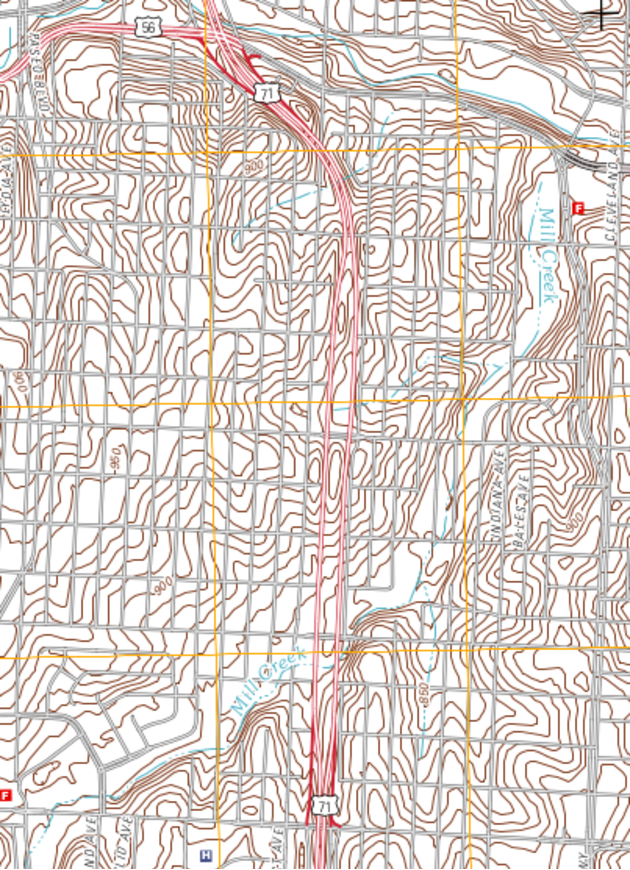
\includegraphics[width=4in]{./images/UR_topo.pdf}}
\end{center}
While a band of dense foliage running from the northeast corner of the corridor to 63\textsuperscript{rd} \& Woodland presents another obstacle, 71 Highway will allow for some longer distance north-south cross connections.

\subsubsection{RF Environment}
The RF enviornment shows light to moderate utilization in the 5GHz band. Our
finding is that while appropriate channel selection and efficiency will be critical,
there is ample spectrum available for use in the target geography. In order to
assess spectrum health, we conducted sector surveys from the roof of the Kelly Center. \par
The graph below reflects the noise and signal levels in the 5GHz spectrum in the direction
of St. Mary's Church, at 31\textsuperscript{st} \& Troost. All but 20MHz worth of spectrum
is deemed usable, with a noise floor well below 90dBm:
\begin{center}
\fbox{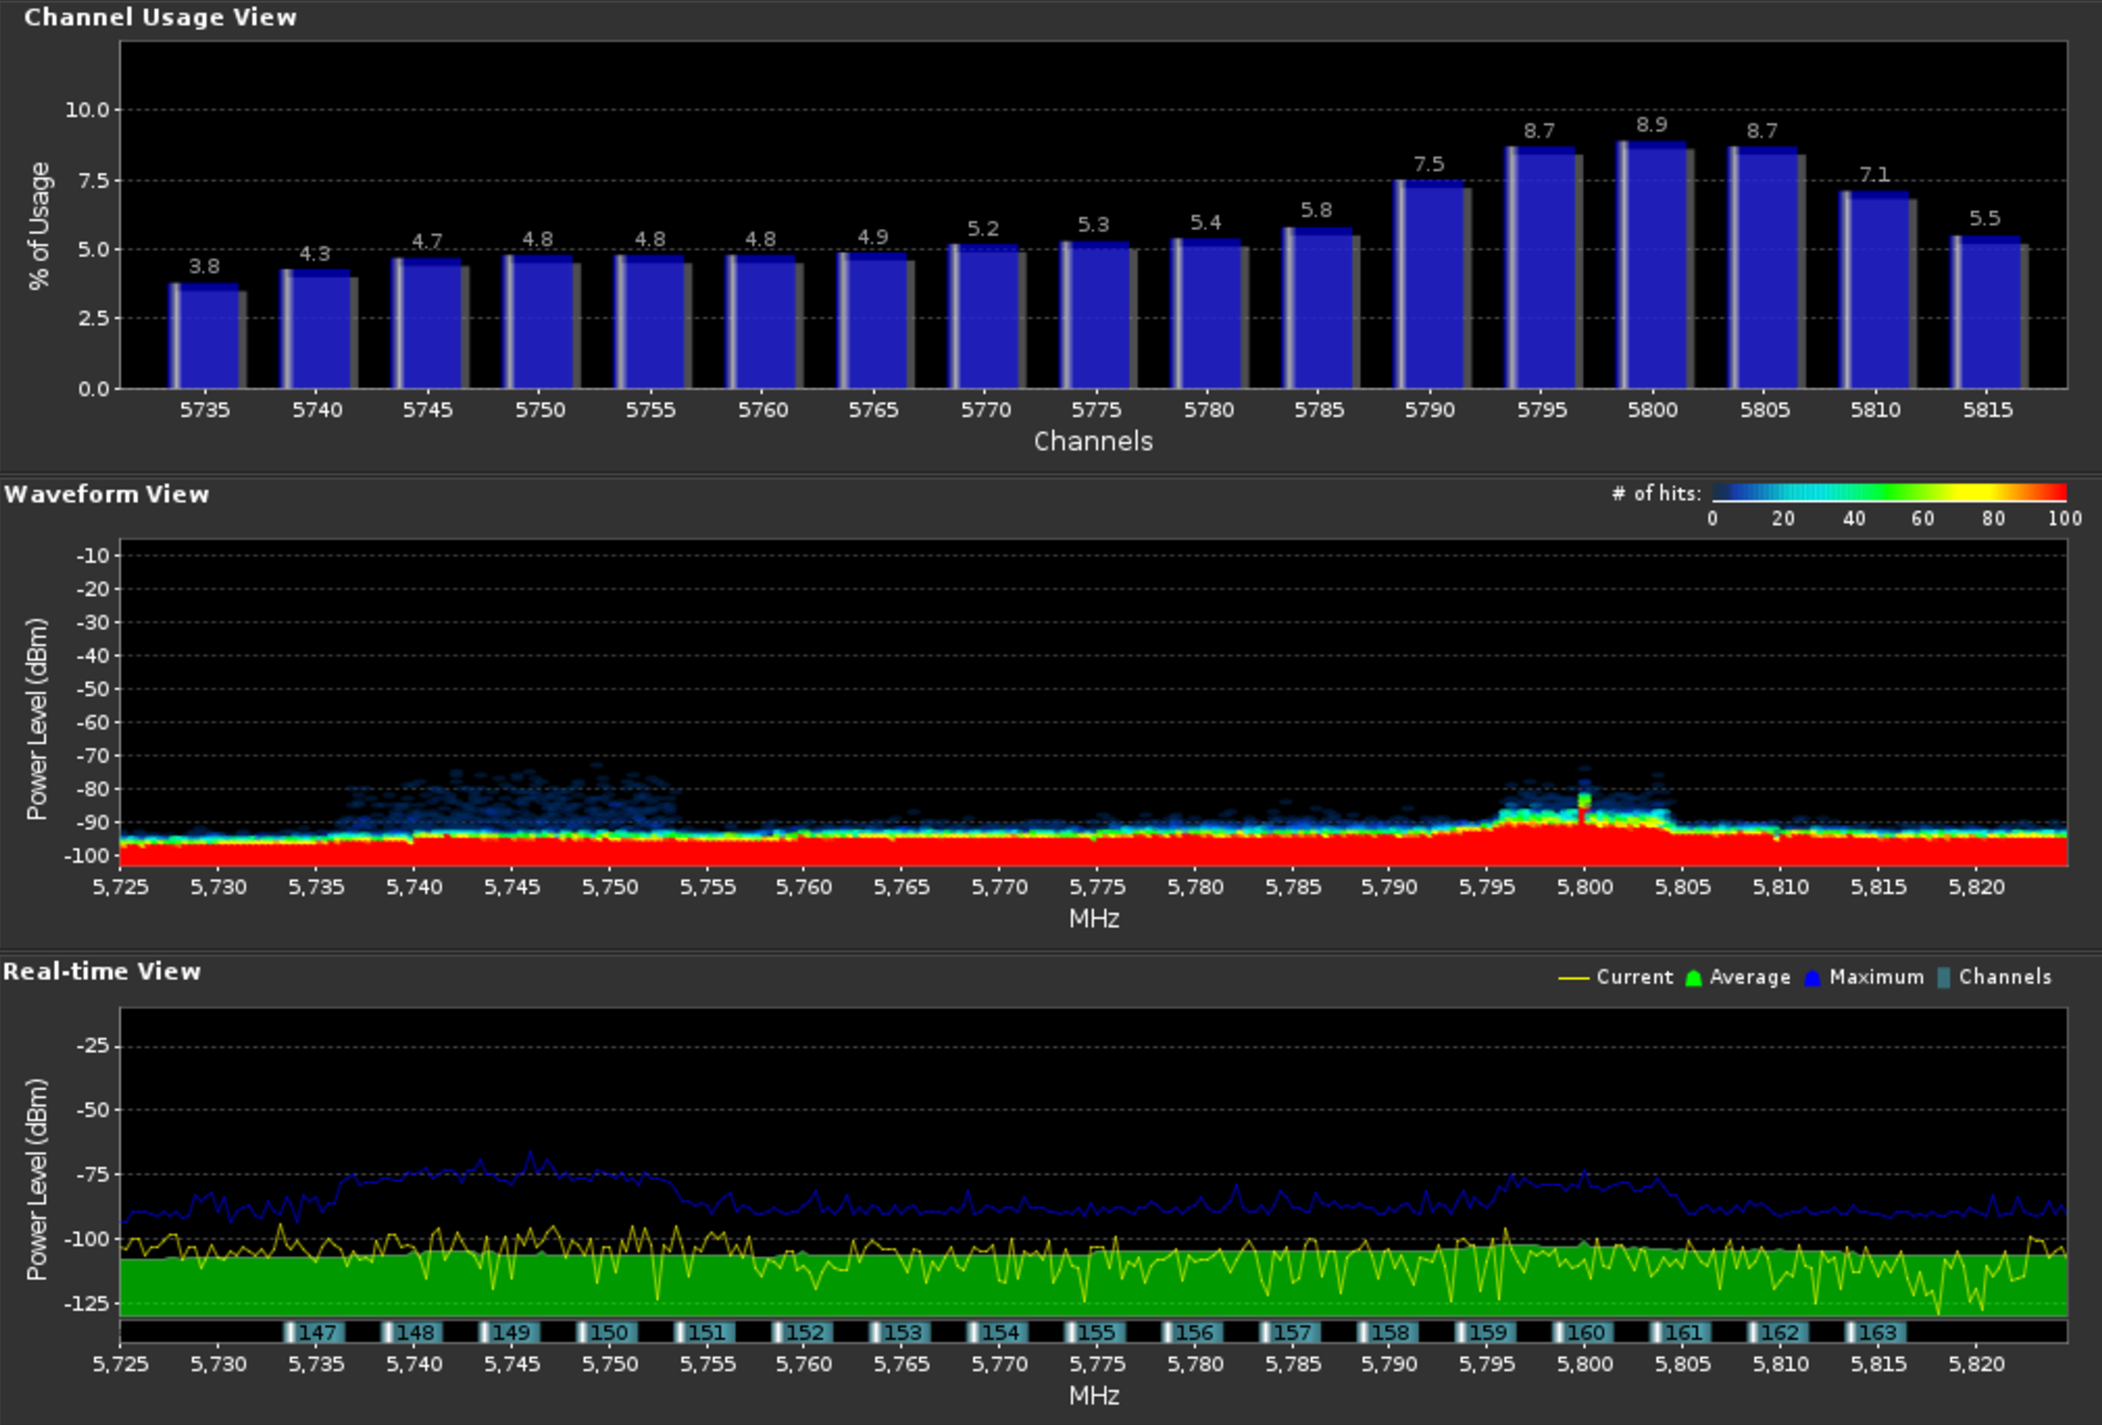
\includegraphics[width=5in]{./images/to3101_rf_airview_crop.pdf}}
\end{center}
The next graph shows the situation in the direction of the DuBois Learning Center, at 
55\textsuperscript{th} \& Cleveland. The spectrum from 5.775GHz to 5.8GHz is not usable, but the rest of the band remains usable:
\begin{center}
\fbox{\includegraphics[width=5in]{./images/to_dubois_airview_crop.pdf}}
\end{center}
Next, in the direction of AC Prep, we see the same sitation as above, with the band from 5.775GHz to 5.8GHz saturated, but the rest of the available frequencies in good shape:
\begin{center}
\fbox{\includegraphics[width=5in]{./images/to_southeasthigh_airview_crop.pdf}}
\end{center}
Finally, looking due west, towards Blue Hills, we see that the entire spectrum is usable, though it does have a slightly higher noise floor, generally approaching 90dBm:
\begin{center}
\fbox{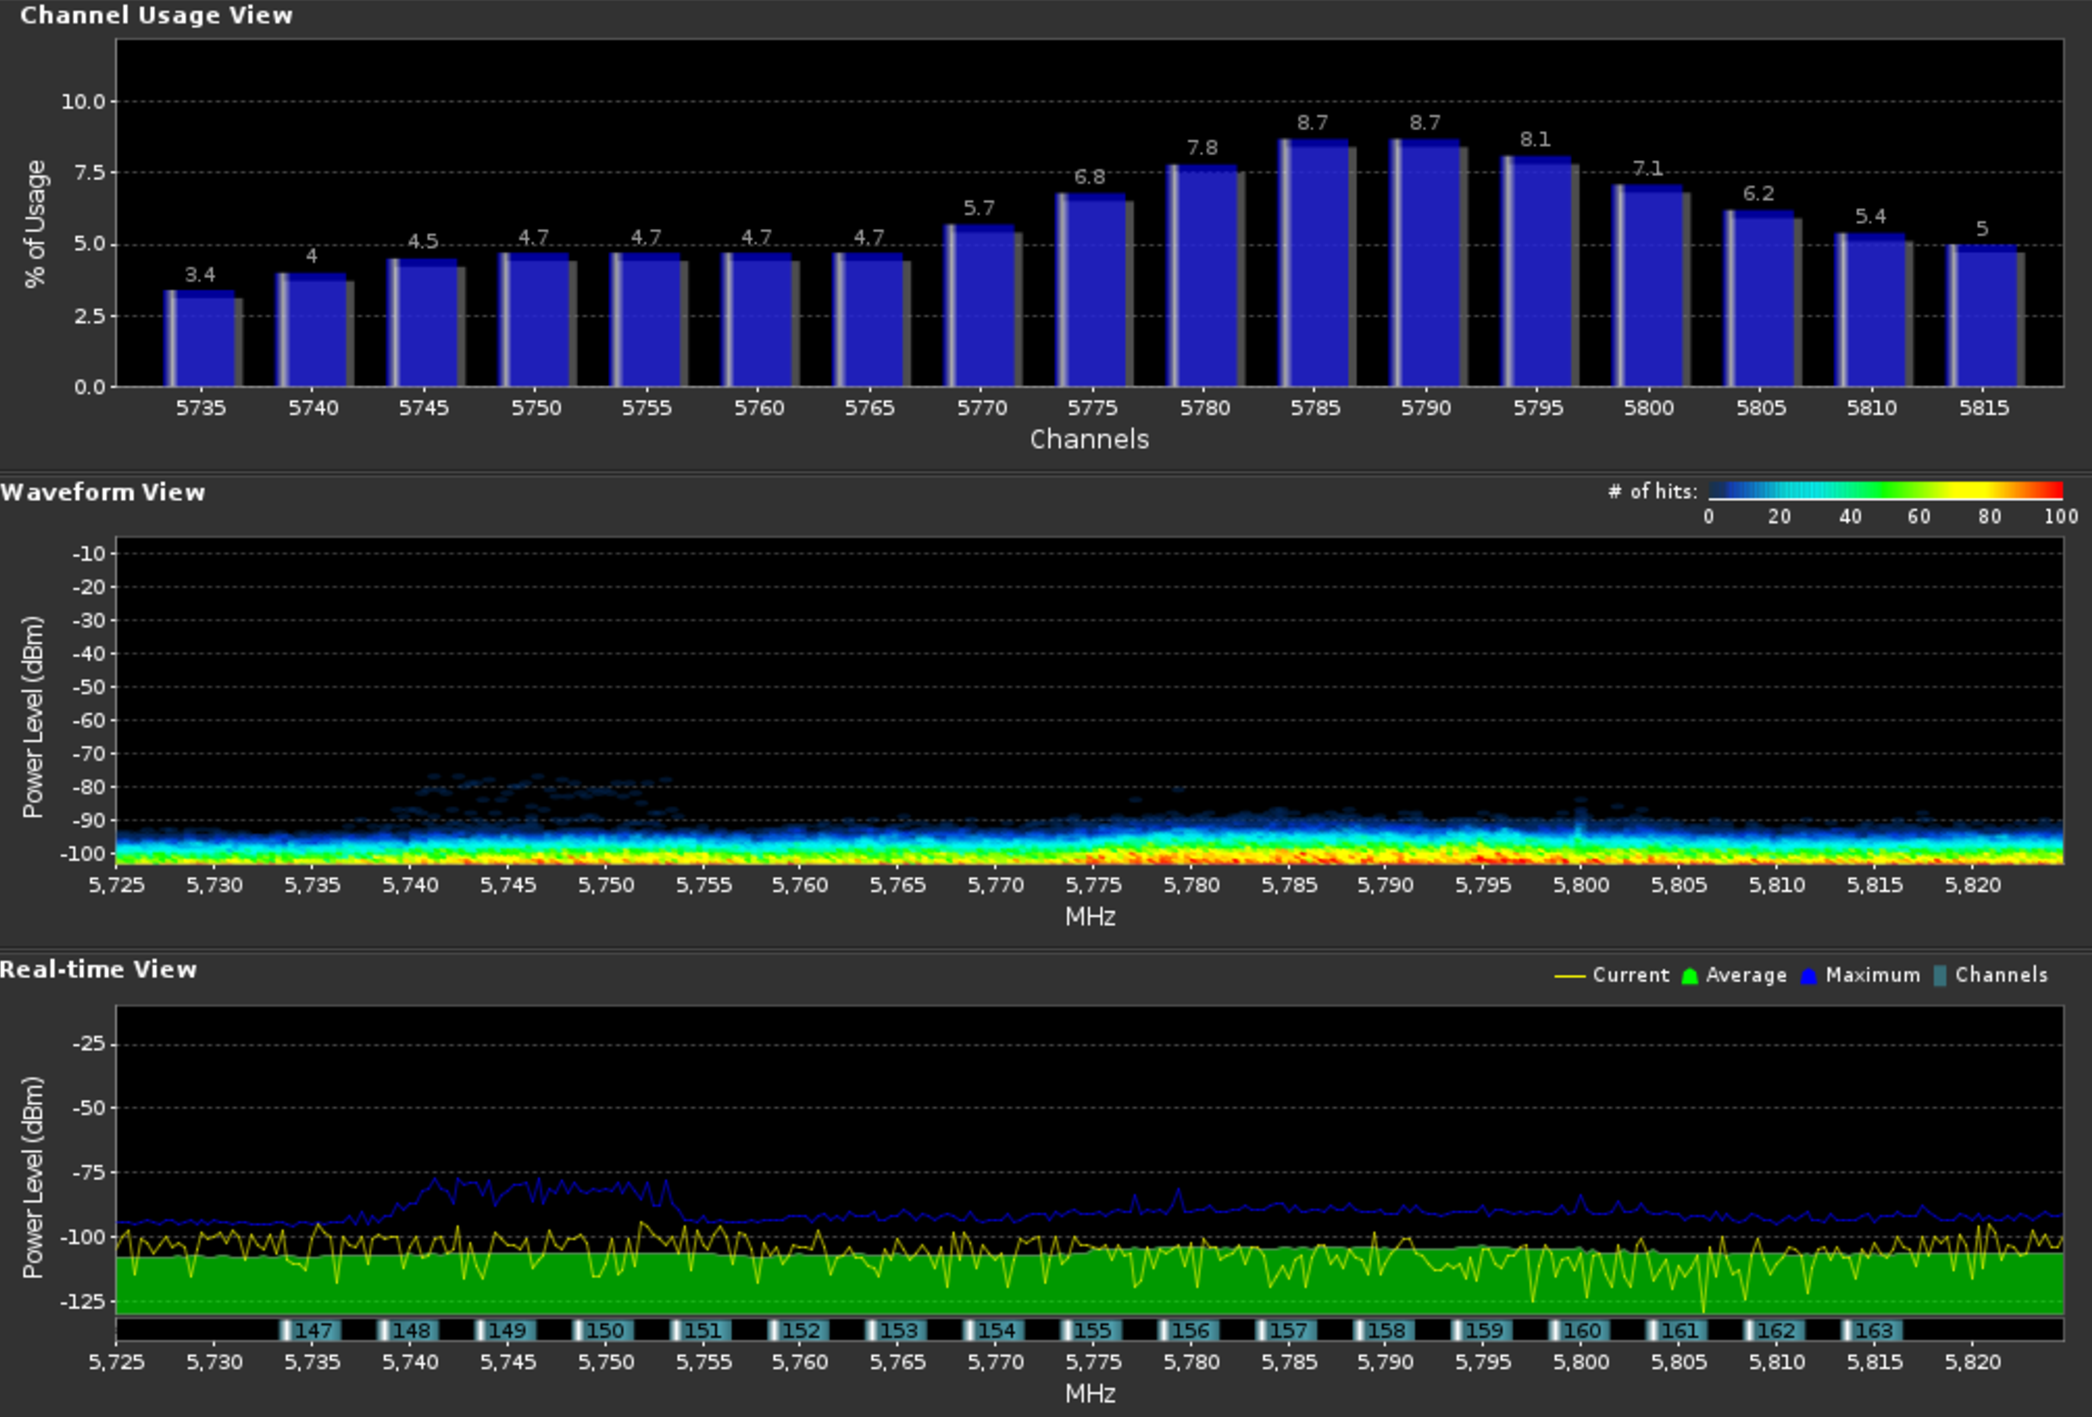
\includegraphics[width=5in]{./images/due_west_airview_crop.pdf}}
\end{center}
We did not survey the 24GHz spectrum that we plan to use for backhaul, because it will be precisely aligned, and should not suffer from interference, as it is not widely deployed.
\subsection{Findings}
On the basis of our survey results and prior field experience, we have devised
a proposed plan of action and associated cost estimates. These projections are intended
to serve as a starting point for collaboration, and certainly do not reflect the
only viable path towards accomplishing the stated objectives.\par
\subsubsection{Proposed Plan}
\begin{description}
\item[Phase I - Spring 2014] As a first phase, we recommend the construction a FreedomTower atop the Mary Kelly Center, and the institution of a community education program designed to teach computer skills. This would immediately create opportunities for block-level organization across much of the footprint. The tower would connect to existing KCFN infrastructure at 31\textsuperscript{st} \& Troost, and would require reengineering 31\textsuperscript{st} \& Troost's existing infrastructure to increase capacity. St. Mary's Church has expressed an openness to such an arrangement, contingent on a roof-rights contract to be negotatiated between The Upper Room and St. Mary's. \par
Ideally, this work would be completed by students and residents, as part of the aforementioned education program, under the guidance of The Free Network Foundation and Connecting for Good. As part of this first phase, it would be necessary to lay the social and political groundwork for further growth. Those involved with the project and education program would reach out directly to potential partners identified in subsequent phases, and to the community at large \par
\item[Phase II - Summer/Fall 2014] Once the Kelly Center tower has been functioning for some time, and a small corps of network volunteers has been stablished, additional towers should be built to expand coverage to the rest of the area. We have identified the DuBois Learning Center and Southeast High School as ideal sites for Phase II construction. With these three towers, virtually all of the blocks in Town Creek, and as many as third of the blocks in Blue Hills would have the abiliy to opt in by constructing a FreedomRelay. Community campaigns to encourage and enable relay construction will be especially important in Blue Hills, where the challenging terrain and lack of tall structures will require the network to expand block-by-block. \par
While it certainly makes sense for community anchor institutions to fund construction of core network infrastructure such as FreedomTowers, and potentially to subsidize the relays and nodes necessary to serve their constituents, long term success depends on a highly distributed ownership model. As such, it will be of critical importance that the network coalition engage in a concerted effort to publicly demonstrate the benefits of the network, and encourage participation. \par

\item[Phase III - 2015 \& Beyond] After the network backbone has been constructed in Phases I and II, the focus should shift entirely to community stakeholdership and organic growth. Those students and community members that have been trained as network technicians should be charged with maintain existing infrastructure and facilitating the construction of new network on a voluntary of commercial basis. \par
At this point, the network would be well situated for expansion to areas outside the scope of this study, espcially to the south and east. Future partners could include libraries, community centers, neighborhood association, additional schools, and all those who recognize the opportunity for mutual benefit inherent in the free network model. \par
\end{description}

\subsubsection{Costs \& Figures}
While the community-driven model has its definite strengths, it can also make it difficult to give precise estimates of cost. Below we present those costs that would be incurred in Phase I, which \emph{can} be immediately quantified.

Phase I one would have the following hard costs:
\begin{center}
\begin{tabular}{|p{5cm}|l|l|l|}
\hline
Item & Q'ty Req'd & Unit Cost & Total Cost \\ \hline
Ubiquiti ToughCable & 2000ft & \$.22/ft & \$220 \\ \hline
Ubiquiti ToughConnectors & 20 & \$.53 & \$10.60 \\ \hline
Ubiquiti ToughSwitch-8 & 1 & \$188 & \$188 \\ \hline
Ubiquiti AirFiber 24 & 4 & \$1,500 & \$6,000 \\ \hline
Ubiquiti NSM5 Loco & 4 & \$70 & \$280 \\ \hline
Glen-Martin 26' Tower & 1 & \$2,561 & \$2,561 \\ \hline
Soekris Net6501-50 & 2 & \$360 & \$720 \\ \hline 
Equipment Rental & 1 & \$2,500 & \$2,500 \\ \hline
Total Hardware & - & - & \$12,479.60 \\ \hline
Labor & - & - & \$10,000 \\ \hline
Support \& Bandwidth & 1 Year & - & \$12,950 \\ \hline
Total & - & - & \$35,429.60 \\ \hline
\end{tabular}
\end{center} 

Build funders reatain complete wonership of all hardware, in accordance with the Network Commons License. The general labor for builds should come from volunteer and student technicians under the supervision of Connecting for Good engineers. Such a volunteer corps would also constitute the first tier of operational support for the network. Connecting for Good will maintain responsibility for keeping the infrastructure up and running, including the provision of gateway bandwidth, for a period of 12 months. After that this responsibility could be transferred to community operators, or a new support contract could be negotatied. \par

By completing Phase I of the above plan, we would lay the groundwork for a high-performance community network in the Swope Corridor. Further investment would necessarily come from a diverse coalition of community stakeholders. By laying the groundwork for the network, and establishing a source of low-cost connectivity, it will become possible to demonstrate the system and bring new participants onboard. We have identified a number of key locations and potential partners, highlighting their locations on the following map: 

\begin{center}
\fbox{\includegraphics[width=4in]{./images/corridor_zoom.jpg}}
\end{center}


A small upfront investment in backbone infrastructure and education, if properly
channeled, has the potential to enable massive, distributed community
improvement. Investing  primarily in know-how, rather than in infrastructure
itself, sets the stage for commercial opportunity, and long-term sustainability.
